%%%%%%%%%%%%%%%%%%%%%%%%%%%%%%%%%%%%%%%%%
% Jacobs Landscape Poster
% LaTeX Template
% Version 1.1 (14/06/14)
%
% Created by:
% Computational Physics and Biophysics Group, Jacobs University
% https://teamwork.jacobs-university.de:8443/confluence/display/CoPandBiG/LaTeX+Poster
% 
% Further modified by:
% Nathaniel Johnston (nathaniel@njohnston.ca)
%
% This template has been downloaded from:
% http://www.LaTeXTemplates.com
%
% License:
% CC BY-NC-SA 3.0 (http://creativecommons.org/licenses/by-nc-sa/3.0/)
%
%%%%%%%%%%%%%%%%%%%%%%%%%%%%%%%%%%%%%%%%%

%----------------------------------------------------------------------------------------
%	PACKAGES AND OTHER DOCUMENT CONFIGURATIONS
%----------------------------------------------------------------------------------------

\documentclass[final]{beamer}

\usepackage{listings}
\usepackage{amsmath}
\usepackage{verbatim}
\usepackage{algorithm}
\usepackage{algorithmic}
\usepackage{etoolbox}
\usepackage{booktabs}
\AtBeginEnvironment{algorithm}{%
  \setlength{\columnwidth}{\linewidth}%
}

\usepackage[scale=1.24]{beamerposter} % Use the beamerposter package for laying out the poster
\usepackage{tipa}
\usepackage{amsmath}
\usepackage{amssymb}
\usepackage{amsfonts}
\usetheme{confposter} % Use the confposter theme supplied with this template
\usepackage{sidecap}
\setbeamercolor{block title}{fg=ngreen,bg=white} % Colors of the block titles
\setbeamercolor{block body}{fg=black,bg=white} % Colors of the body of blocks
\setbeamercolor{block alerted title}{fg=white,bg=dblue!70} % Colors of the highlighted block titles
\setbeamercolor{block alerted body}{fg=black,bg=dblue!10} % Colors of the body of highlighted blocks
% Many more colors are available for use in beamerthemeconfposter.sty

%-----------------------------------------------------------
% Define the column widths and overall poster size
% To set effective sepwid, onecolwid and twocolwid values, first choose how many columns you want and how much separation you want between columns
% In this template, the separation width chosen is 0.024 of the paper width and a 4-column layout
% onecolwid should therefore be (1-(# of columns+1)*sepwid)/# of columns e.g. (1-(4+1)*0.024)/4 = 0.22
% Set twocolwid to be (2*onecolwid)+sepwid = 0.464
% Set threecolwid to be (3*onecolwid)+2*sepwid = 0.708

\usepackage{pifont}% http://ctan.org/pkg/pifont
\newcommand{\cmark}{\ding{51}}%
\newcommand{\xmark}{\ding{55}}%
\usepackage{dsfont}

\newtheorem{proposition}{Proposition}
\newcommand{\expect}{\mathds{E}} %{{\rm I\kern-.3em E}}
\newcommand{\probability}{\mathds{P}} %{{\rm I\kern-.3em P}}
\newcommand{\indicator}{\mathds{1}} %{{\rm I\kern-.3em P}}

%\newtheorem{definition}{Definition}

\newlength{\sepwid}
\newlength{\onecolwid}
\newlength{\twocolwid}
\newlength{\threecolwid}
\setlength{\paperwidth}{96in} % A0 width: 46.8in
\setlength{\paperheight}{48in} % NIPS16 : 36
\setlength{\sepwid}{0.024\paperwidth} % Separation width (white space) between columns
\setlength{\onecolwid}{0.22\paperwidth} % Width of one column
\setlength{\twocolwid}{0.464\paperwidth} % Width of two columns
\setlength{\threecolwid}{0.708\paperwidth} % Width of three columns
\setlength{\topmargin}{-0.5in} % Reduce the top margin size
%-----------------------------------------------------------

\usepackage{etoolbox}
\makeatletter
\patchcmd{\beamer@@tmpl@headline}{wd=47in}{wd=95in}{}{}
\makeatother

\usepackage{graphicx}  % Required for including images
\usepackage{verbatim}
\usepackage{booktabs} % Top and bottom rules for tables
\usepackage{fancyvrb}
\DeclareMathOperator*{\argmin}{arg\,min} % thin space, limits underneath in displays
% \DeclareMathOperator{\argmin}{argmin} % no space, limits underneath in displays
\DeclareMathOperator*{\argmax}{arg\,max} % thin space, limits underneath in displays
% \DeclareMathOperator{\argmax}{argmax} % no space, limits underneath in displays

\newcommand{\expect}{\mathds{E}} %{{\rm I\kern-.3em E}}
\newcommand{\probability}{\mathds{P}} %{{\rm I\kern-.3em P}}
\newcommand{\indicator}{\mathds{1}} %{{\rm I\kern-.3em P}}

\begin{SaveVerbatim}[]{ListSketch}
Program ::=
  (if Bool List
    (append RecursiveList
            RecursiveList
            RecursiveList))
Bool ::= (<= Int) | (>= Int)
Int  ::= 0 | (1+ Int) | (1- Int)
       | (length List) | (head List)
List ::= nil | (filter Bool List)
      | X | (tail List) | (list Int)
RecursiveList ::= List
                | (recurse List)
\end{SaveVerbatim}

\begin{SaveVerbatim}[]{TextSketch}
Program ::= Term | Program + Term
Term    ::= String | substr(Pos,Pos)
Pos     ::= Number
         |  pos(String,String,Number)
Number  ::= 0 | 1 | 2 | ... 
         | -1 | -2 | ...
String  ::= Character 
         |  Character + String
Character ::= a | b | c | ...
\end{SaveVerbatim}



\usepackage{wrapfig}

%----------------------------------------------------------------------------------------
%	TITLE SECTION 
%----------------------------------------------------------------------------------------
\usepackage{stmaryrd}
\newcommand{\tuple}[1]{\ensuremath{\left \langle #1\right \rangle}}
\newcommand{\sem}[1]{[\mkern-6mu[#1]\mkern-6mu]} %\newcommand{\sem}[1]{\llbracket #1\rrbracket}

\usetikzlibrary{trees}
\usetikzlibrary{fit}
\usetikzlibrary{calc}
\usetikzlibrary{bayesnet}

\usepackage{arydshln}

\usepackage[normalem]{ulem}
\newcommand{\theSystem}{\textsc{DreamCoder}}
\title{Learning to Infer Graphics Programs from Hand-Drawn Images} % Poster title

\author{Kevin Ellis, Daniel Ritchie, Armando Solar-Lezama,  Joshua B. Tenenbaum} % Author(s)

\institute{Massachusetts Institute of Technology \& Brown University} % Institution(s)

%----------------------------------------------------------------------------------------

\begin{document}
\addtobeamertemplate{headline}{} 
{\begin{tikzpicture}[remember picture, overlay]
     \node [anchor=north east, inner sep=3cm]  at ([yshift=2cm]current page.north east)
           {\includegraphics[height=10cm]{figures/Brown.png}};
                \node [anchor=north west, inner sep=3cm]  at (current page.north west)
     {\includegraphics[height=7cm]{figures/csail.png}};
\end{tikzpicture}}

\addtobeamertemplate{block end}{}{\vspace*{2ex}} % White space under blocks
\addtobeamertemplate{block alerted end}{}{\vspace*{2ex}} % White space under highlighted (alert) blocks

\setlength{\belowcaptionskip}{2ex} % White space under figures
\setlength\belowdisplayshortskip{2ex} % White space under equations

\begin{frame}[t] % The whole poster is enclosed in one beamer frame

\begin{columns}[t] % The whole poster consists of three major columns, the second of which is split into two columns twice - the [t] option aligns each column's content to the top

\begin{column}{\sepwid}\end{column} % Empty spacer column

\begin{column}{\onecolwid} % The first column

%----------------------------------------------------------------------------------------
%	OBJECTIVES
%----------------------------------------------------------------------------------------

  \begin{alertblock}{Hand drawings to high-level graphics procedures}
    Convert image of hand drawing into $\LaTeX$ (left pair: top white is drawing, bottom black is $\LaTeX$ render). Infer high-level graphics program from drawing: captures higher-order structure like repetition, motifs, symmetries.
    \includegraphics[width = \textwidth]{firstPageExample.pdf}
\end{alertblock}

      \begin{block}{Example System Outputs}
\includegraphics[width = \textwidth]{examplePrograms.pdf} 
      \end{block}

      \begin{alertblock}{\red Acknowledgments}
         We are grateful for advice from Will Grathwohl and Jiajun Wu on  the neural architecture. Funding from NSF GRFP, NSF Award 
\#1753684, the MUSE program (DARPA grant FA8750-14-2-0242),
and AFOSR award FA9550-16-1-0012.
        \end{alertblock}

%----------------------------------------------------------------------------------------
%	INTRODUCTION
%----------------------------------------------------------------------------------------



%% \begin{block}{Problem Framing}
%%   \begin{itemize}
%%   \item Sketch specifies a large but finite set of programs, $S$
%%   \item Program description length: $\lvert x \rvert$ for $x\in S$
%%   \item Prior over programs: $\propto 2^{- \lvert x \rvert }$
%%   \item Posterior over programs: call this $p(x)$, defined as $\propto 2^{- \lvert x \rvert } \mathds{1}[x \text{ consistent with input/output examples}]$
%%   \end{itemize}
%%   Our goal then  is to sample from $p(\cdot)$.
%% \end{block}



%------------------------------------------------



%----------------------------------------------------------------------------------------

\end{column} % End of the first column

\begin{column}{\sepwid}\end{column} % Empty spacer column

\begin{column}{\twocolwid} % Begin a column which is two columns wide (column 2)

  \begin{block}{Two-Stage Pipeline}
\centering  \includegraphics[width = 80cm]{pipeline.pdf}
  
  Black arrows: Top--down generative model; Program$\to$Spec$\to$Image. {\color{red}Red} arrows: Bottom--up inference procedure. \textbf{Bold:} Random variables (image/spec/program)
\end{block}

\begin{columns}[t,totalwidth=\twocolwid] % Split up the two columns wide column

\begin{column}{\onecolwid}\vspace{-.6in} % The first column within column 2 (column 2.1)

%----------------------------------------------------------------------------------------
%	MATERIALS
%----------------------------------------------------------------------------------------
%

%%  \begin{alertblock}{Bayesian Program Learning \& other approaches} %
    %% Why might a learner represent knowledge as a program,
    %% rather than the representations popular in much of machine learning,
    %% such as a large matrix of weights or a graphical model?
    %% Programs (probabilistic or deterministic)
    %% excel at representing knowledge that is (1) symbolic; (2) compositional; or (3) higher-order.
    %% We are motivated by the success of program induction
    %% in both AI domains,
    %% like semantic parsing and programming by demonstration,
    %% and in cognitive modeling,
    %% like intuitive theory learning~\cite{logical}.
%%\end{alertblock}
  
\begin{block}{Parsing Images into Drawing Commands (specs)}
\hspace{10cm}  \includegraphics[width = 40cm]{architecture.pdf}

{\small   \textcolor{blue}{Blue}: network inputs. Black: network operations. \textcolor{red}{Red}: draws from a multinomial. \texttt{Typewriter font}: network outputs. Renders on a $16\times 16$ grid, shown in \textcolor{gray}{gray}. STN: differentiable attention mechanism. \textbf{Combined with stochastic search (Sequential Monte Carlo)}}

\end{block}

\begin{block}{Generalizing to real hand drawings}
  \textbf{  Train on simulated noisy data (left) \& learn distance metric between images (right)}\\
  \newcommand{\noisySize}{0.2\textwidth}
  \begin{minipage}[t]{\noisySize}
    \centering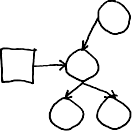
\includegraphics[width = \textwidth]{figures/expert-60-reduced.png}\\
{\small     (a): hand drawing}
  \end{minipage}%
  \begin{minipage}[t]{\noisySize}
    \centering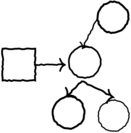
\includegraphics[width = \textwidth]{figures/60-1-reduced.png}\\
{\small     (b): noisy render of (a)}
  \end{minipage}\hfill%
  \begin{minipage}[t]{0.5\textwidth}\vspace{-9cm}
    \textbf{Learned distance metric}\\
    Serves as likelihood surrogate for SMC
      \begin{align*}
    -\log L_{\text{learned}}(\text{render}&(S_1)|\text{render}(S_2))\approx\\& |S_1 - S_2| + |S_2 - S_1|\label{symmetricDistance}
      \end{align*}
      $S_1$: noisy render of random scene\\
      $S_2$: nonnoisy render of random scene
  \end{minipage}%

  \vspace{3cm}

    \begin{minipage}[c]{0.49\textwidth} 
    \centering  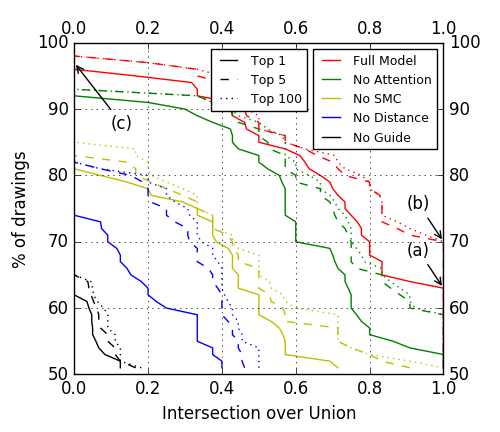
\includegraphics[width = \textwidth]{figures/drawingAccuracy.png}            \vspace{-0.5cm} 
  \end{minipage}\hfill%
      \begin{minipage}[c]{0.5\textwidth} 
  {\small (Left) NN outputs vs ground truth on hand drawings (measured by IoU), as we consider larger sets of samples (1, 5, 100).
     (a) for 63\% of drawings the model's top prediction is exactly correct; (b) for 70\% of drawings the ground truth is in the top 5 model predictions; (c) for 4\% of drawings all of the model outputs have no overlap with the ground truth. Red: the full model. Other colors: ablations. Model is at ceiling for synthetic $\LaTeX$ output.}
      \end{minipage}

  \end{block}



%----------------------------------------------------------------------------------------

\end{column} % End of column 2.1

\begin{column}{\onecolwid}\vspace{-.6in} % The second column within column 2 (column 2.2)

%----------------------------------------------------------------------------------------
%	METHODS
%----------------------------------------------------------------------------------------



  \begin{block}{Domain-Specific Language for Graphics Programs}
 We allow loops (\texttt{for}) with conditionals (\texttt{if}), vertical/horizontal reflections (\texttt{reflect}), variables (Var) and affine transformations ($\mathbb{Z}\times$Var\texttt{+}$\mathbb{Z}$).
  \begin{tabular}{rl}\toprule
  Program$\to$&Statement; $\cdots$; Statement\\
  Statement$\to$&\texttt{circle}(Expression,Expression)\\
  Statement$\to$&\texttt{rectangle}(Expression,Expression,Expression,Expression)\\
  Statement$\to$&\texttt{line}(Expression,Expression,Expression,Expression,Boolean,Boolean)\\
  Statement$\to$&\texttt{for}$(0\leq \text{Var}  < \text{Expression})$\texttt{ \{ if }$(\text{Var} > 0)$\texttt{ \{ }Program\texttt{ \}; }Program\texttt{ \}}\\
  Statement$\to$&\texttt{reflect}$(\text{Axis})$\texttt{ \{ }Program\texttt{ \}}\\
  Expression$\to$&$\mathbb{Z}\times$Var\texttt{+}$\mathbb{Z}$\\
%  Var$\to$&A free (unused) variable\\
  Axis$\to$&\texttt{X = }$\mathbb{Z}$ | \texttt{Y = }$\mathbb{Z}$\\
    $\mathbb{Z}\to$&an integer\\\bottomrule
  \end{tabular}
  \end{block}

  \begin{block}{Learning \& Constraint-Based Program Synthesis}
    \textbf{Sketch}: state-of-the-art program synthesizer. Solar-Lezama 2008.\\Solves, for spec $S$ \& program $p$:
$$
  \text{program}(S) = \argmin_{p\in \text{DSL, s.t. }p \text{ consistent w/ } S} \text{cost}(p)\label{programObjective}
$$
  \textbf{Learn policy $\pi_\theta$ to accelerate program synthesizer's search.}\\ $\pi_\theta(\cdot |S) \in  \Delta^\Sigma$,
  where $\Sigma\ni\sigma $ a set of synthesis problem (i.e., $\sigma \in \Sigma $ is a sketch)

%%   \noindent\textbf{Definition: Bias-optimality.}  (c.f. Schmidhuber 2004)
%%    A search algorithm is $n$-\emph{bias optimal}
%% with respect to a distribution $\probability_{\text{bias}}[\cdot ]$ if it is
%% guaranteed to find a solution in $\sigma $ after searching for at least time
%% $n\times\frac{t(\sigma )}{\probability_{\text{bias}}[\sigma ]}$, where $t(\sigma )$ is the time it
%% takes to verify that $\sigma $ contains a solution to the
%% search problem.

%% Here, $\probability_{\text{bias}}[\cdot ] = \pi_\theta(\cdot |S)$.
\textbf{Inference strategy}: Timeshare according to $\pi_\theta(\cdot |S)$, like in Levin Search
  \begin{figure}\centering
  \begin{tikzpicture}[scale=3]
    \node[anchor = west] at (0,5.25) {Entire program search space};
    \draw[fill = yellow,fill opacity = 0.15,draw = black] (0,0) rectangle (5,5);
    \draw [fill = yellow, opacity = 0.2] (0,0)--(0,2)--(4,0)--(0,0);
    \draw [fill = yellow, opacity = 0.4,cycle] (0,5)--(0,1)--(3,5);
    \draw [fill = yellow, opacity = 0.6,cycle] (2.5,5)--(3.2,0)--(5,0)--(5,5);
    \draw (0,2) -- node[below,sloped]{short programs} (4,0);
    \draw (0,2) -- node[above,sloped]{long programs} (4,0);
    \draw (2.5,5) -- node[above,sloped]{programs w/ reflections} (3.2,0);
    \draw (0,1) -- node[above,sloped]{ programs w/ loops} (3,5);
    \node(p1)[anchor =west ] at (5.5,3.5) {$\pi_\theta(\text{short, no loop/reflect}) = $};
    \draw [fill = yellow, fill opacity = 0.2,draw = black]  ([xshift = 0cm,yshift = -0.2cm]p1.east) rectangle ([xshift = 0.4cm,yshift = 0.2cm]p1.east);
    \node(p2)[anchor =west ] at ([yshift = -0.5cm]p1.west) {$\pi_\theta(\text{long, loops}) = $};
    \draw [fill = yellow, fill opacity = 0.4,draw = black]  ([xshift = 0cm,yshift = -0.2cm]p2.east) rectangle ([xshift = 0.4cm,yshift = 0.2cm]p2.east);
    \node(p3)[anchor =west ] at ([yshift = -0.5cm]p2.west) {$\pi_\theta(\text{long, no loop/reflect}) = $};
    \draw [fill = yellow, fill opacity = 0.15,draw = black]  ([xshift = 0cm,yshift = -0.2cm]p3.east) rectangle ([xshift = 0.4cm,yshift = 0.2cm]p3.east);
    \node(p4)[anchor =west ] at ([yshift = -0.5cm]p3.west) {$\pi_\theta(\text{long, reflects}) = $};
    \draw [fill = yellow, fill opacity = 0.6,draw = black]  ([xshift = 0cm,yshift = -0.2cm]p4.east) rectangle ([xshift = 0.4cm,yshift = 0.2cm]p4.east);
    \node(p5)[anchor =west ] at ([yshift = -0.5cm]p4.west) {\emph{etc.}};
  \end{tikzpicture}
  \caption{The bias-optimal search algorithm divides the entire (intractable) program search space in to (tractable) program subspaces (written $\sigma $), each of which contains a restricted set of programs. For example, one subspace might be short programs which don't loop. The policy $\pi$ predicts a distribution over program subspaces:  weight assigned by $\pi$ indicated by  shading}
\end{figure}

Differentiable loss ($\mathcal{D}$ a corpus of synthesis problems):
\begin{align}
\textsc{Loss}(\theta ; \mathcal{D})& =  \expect_{S\sim\mathcal{D}}\left[ \min_{\sigma\in \text{\textsc{Best}}(S)}\frac{t(\sigma | S)}{\pi_\theta (\sigma | S)}\right] + \lambda \Vert\theta\Vert_2^2\label{policyLoss}\\
\text{where }  \sigma \in\text{\textsc{Best}}(S) &\text{ if  a minimum cost program for }S \text{ is in }\sigma .\nonumber %\text{cost}(\text{program}(p)) = \min_{p\in \sigma \text{, s.t. }p\text{ evaluates to }S} \text{cost}(p) \nonumber
\end{align}

\begin{flushright}
  Experimental results on synthesis policy: See lower right of poster
  \end{flushright}

  \end{block}

%----------------------------------------------------------------------------------------

\end{column} % End of column 2.2

\end{columns} % End of the split of column 2 - any content after this will now take up 2 columns width


%----------------------------------------------------------------------------------------

\begin{columns}[t,totalwidth=\twocolwid] % Split up the two columns wide column again

 % End of column 2.1

\begin{column}{\onecolwid} % The second column within column 2 (column 2.2)

%----------------------------------------------------------------------------------------
%	RESULTS
%----------------------------------------------------------------------------------------


%----------------------------------------------------------------------------------------

\end{column} % End of column 2.2

\end{columns} % End of the split of column 2

\end{column} % End of the second column

\begin{column}{\sepwid}\end{column} % Empty spacer column

\begin{column}{\onecolwid} % The third column

%----------------------------------------------------------------------------------------
%	CONCLUSION
%----------------------------------------------------------------------------------------

  \begin{block}{Extrapolating Drawings}
    Automatically extrapolate by increasing loop bounds. Top white: Hand drawing. Bottom black: extrapolation.
    
      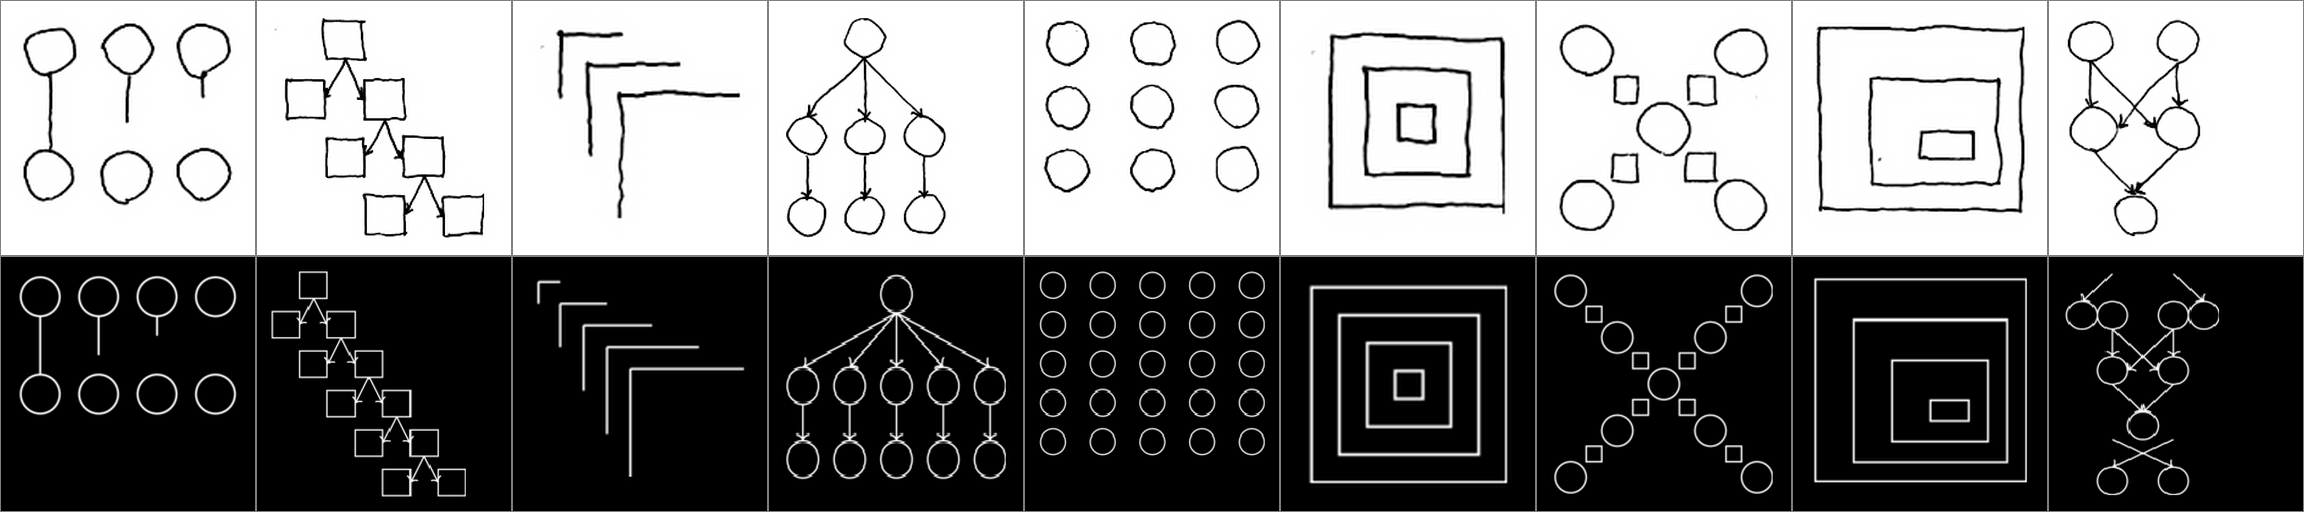
\includegraphics[width = \textwidth]{figures/extrapolationMatrix1.png}\\
  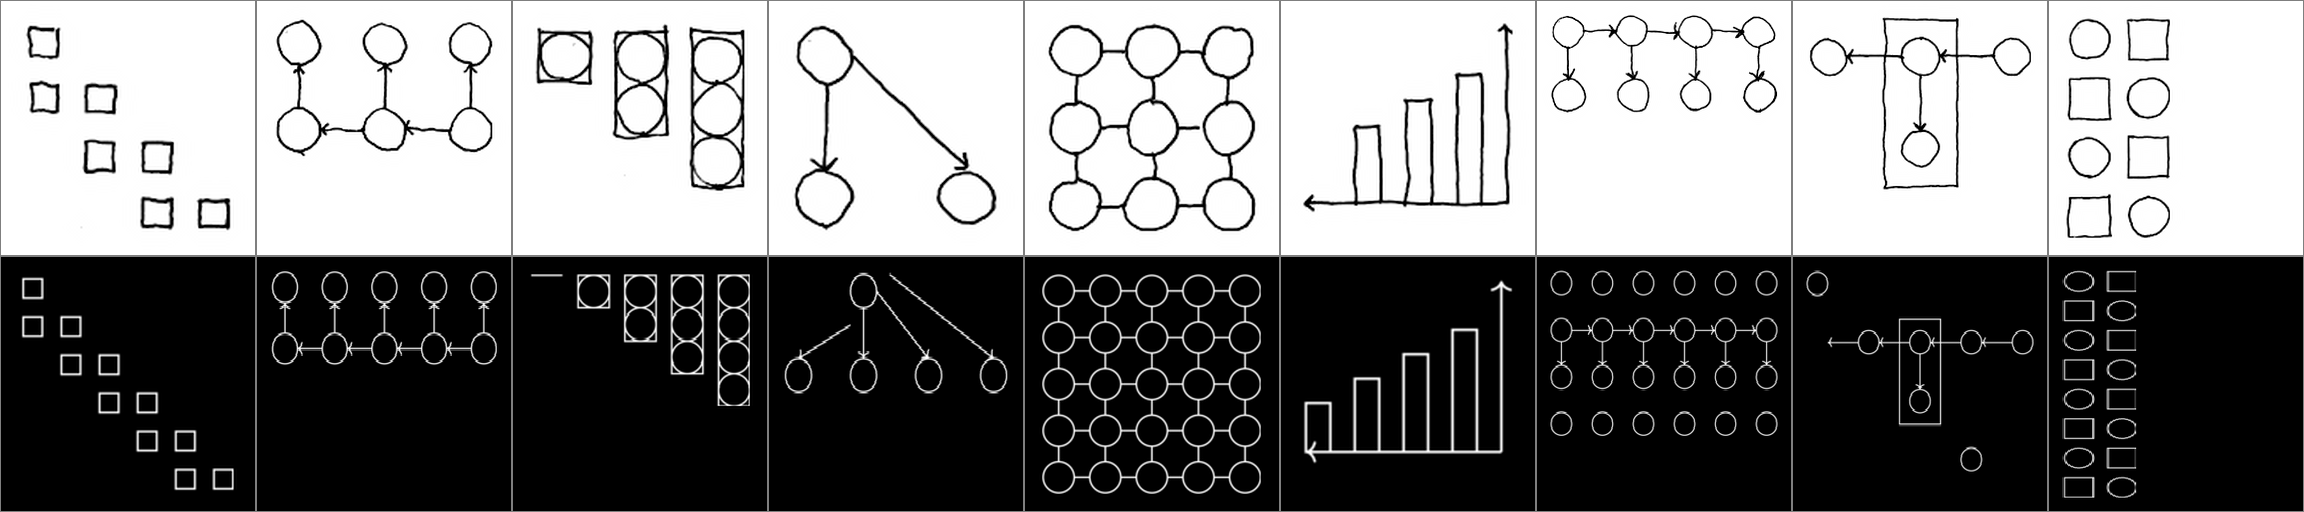
\includegraphics[width = \textwidth]{figures/extrapolationMatrix2.png}\\
  \includegraphics[width = \textwidth]{figures/extrapolationMatrix3.png}  \\
  \end{block}

  \begin{block}{Error correction}
    `Top down' influences upon perception: reasoning engine (program synthesizer) can influence
    agent's percept through higher-level considerations like symmetry and alignment.
    \begin{align*}
      \hat{S}(I) &= \argmax_{S\in \mathcal{F}(I)} L_{\text{learned}}(I | \text{render}(S))\times \probability_\theta[S|I] \times\probability_{\beta} [ \text{program}(S)] \\
        \beta^* &= \argmax_{\beta} \expect \left[ \log \frac{\probability_{\beta} [\text{program}(S)]\times L_{\text{learned}}(I|\text{render}(S))\times \probability_\theta[S|I]}{\sum_{S'\in \mathcal{F}(I)} \probability_{\beta} [\text{program}(S')]\times L_{\text{learned}}(I|\text{render}(S'))\times \probability_\theta[S'|I]} \right]
    \end{align*}
    where $\mathcal{F}(I)$ is set of parses output by neural net on image $I$;
    $\probability_\beta[\cdot ]$ is prior over programs parameterized by $\beta$;
    and expectation is taken over a corpus of
    program synthesis problems.

    \vspace{2cm}
    \begin{figure}
        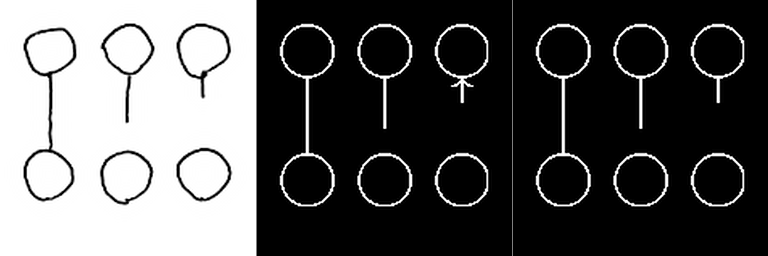
\includegraphics[width = 0.5\textwidth]{figures/programSuccess7.png}\\
  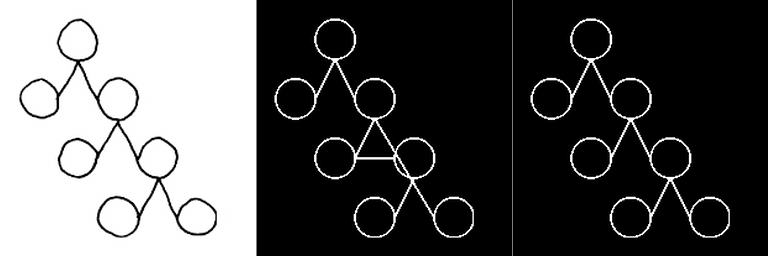
\includegraphics[width = 0.5\textwidth]{figures/programSuccess16.png}
  \caption{Left: hand drawings. Center: interpretations favored by the deep network. Right: interpretations favored after learning a prior over programs. The prior favors  simpler programs, thus (top) continuing the pattern of not having an arrow is preferred, or (bottom) continuing the ``binary search tree'' is preferred.}
    \end{figure}
\vspace{-1cm}
  \end{block}

  \begin{block}{Synthesis times}    
    \includegraphics[width = \textwidth]{figures/policyComparison_basic_DC+bias_20.png}

{\small Time to synthesize a minimum cost program. Sketch: out-of-the-box performance of Sketch. DC: Deep--Coder style baseline that predicts program components, trained like Balog 2016. Oracle:  upper bounds  the performance of any bias--optimal search policy. $\infty = $ timeout. Red dashed line is median time}
    \end{block}


%----------------------------------------------------------------------------------------
%	REFERENCES
%----------------------------------------------------------------------------------------

\setbeamercolor{block title}{fg=red,bg=white} % Change the block title color
%% \begin{block}{References}

%%   %\nocite{*} % Insert publications even if they are not cited in the poster
%%   \renewcommand{\refname}{\vspace{-0.8em}}
%%           \bibliographystyle{plain}
%%           \bibliography{main}
%% %\small{\bibliographystyle{plain}
%% %\bibliography{main}}

%% \end{block}

%----------------------------------------------------------------------------------------
%	ACKNOWLEDGEMENTS
%----------------------------------------------------------------------------------------

\setbeamercolor{block title}{fg=red,bg=white} % Change the block title color

%% \begin{block}{Acknowledgements}

%% \small{\rmfamily{We are grateful for feedback from Adam Smith, Kuldeep Meel, and our anonymous reviewers.
%% Work supported by AFOSR award FA9550-16-1-0012.}} \\

%% \end{block}

%----------------------------------------------------------------------------------------
%	CONTACT INFORMATION
%----------------------------------------------------------------------------------------


%----------------------------------------------------------------------------------------

\end{column} % End of the third column

\end{columns} % End of all the columns in the poster

\end{frame} % End of the enclosing frame

\end{document}

